\chapter{Introduction}\label{C:intro}
\section{Problem Statement}
% \textcolor{Blue}{You should make a decision on the topic you want to achieve. \\
	% Energy Efficient Cloud Resources Allocation with Container-based Cloud Computing}\\
% \textcolor{Maroon}{General introduction of cloud computing and Energy Consumption problem}
% The energy consumption in a data center has become the major concern for a Cloud provider. 

% The energy wastage mainly comes from the unproportional use of server resources \cite{Barroso:2007jt}

% Server consolidation \cite{Zhang:2010vo} is the major strategy to resolve this issue. 
% It reduces the server energy consumption by gathering virtual machines (VMs) into a fewer 
% number of physical servers so that idle servers can be turned off. 
\textcolor{Blue}{Cloud computing definition}\\
Cloud computing is a computing model offers a network of servers to their 
clients in a on-demand fashion. From NIST's definition \cite{Mell:2011jj}, \textit{"cloud computing is a model for enabling ubiquitous, convenient, on-demand network access to a shared pool of configurable computing resources (e.g., networks, servers, storage, applications and services) that can be rapidly provisioned and released with minimal management effort or service provider interaction."}

\textcolor{Blue}{Cloud computing advantages}\\
Cloud computing has completely reformed the software industry \cite{Buyya:2009ix} by providing three major benefits to web-based software or web service providers.
First, service providers do not need upfront investment in hardwares (e.g servers and networking devices) and pay for hardwares' maintenance. 
Second, service providers will not worried about the limited resources will obstruct the performance of their services when unexpected high demand occurs. The elastic nature of cloud can dynamic allocate and release resources for a service. In addition, software providers can pay as much as the resource usage under a \emph{pay-as-you-go} policy.
Third, service providers can publish and update their applications at any location 
as long as there is an Internet connection. 
These advantages allow anyone or organization to deploy their softwares on Cloud in
a reasonable price. 
% Cloud computing involves with three actors:
% \emph{Cloud provider}, \emph{Cloud users} and \emph{End users} 
% \cite{}. Cloud providers build and maintain the infrastructure of Cloud data centers. 
% Cloud users lease resources such as virtual machines from Cloud providers to deploy their applications so that end users can buy their services.

% The convenience offered by Cloud computing and the 
% difficulties of managing Cloud resources are two sides of a coin. 
\textcolor{Blue}{Research Problem}\\
From Cloud providers' perspective, they are trying to make the most profit on data centers.
On one hand, cloud providers are trying to improve the quality of  Cloud service to attractive more service providers migrate their business to Cloud.  
On the other hand, they want to cut enormous energy consumption 
- as much as 25,000 households \cite{Kaplan:up01fR-k} - to lower the expense. 

Energy consumption in data centers are derived from several parts as 
illustrated in Figure \ref{fig:consumption}. 
Regardless the energy consumption of refrigeration system (or cooling system), 
the majority of energy consumption are from servers. 
According to Hameed et al \cite{Hameed:2016cma}, 
servers are far from energy-efficient and 
the main reason for its wastage is ``the idle power when ICT resources such as servers providing computing and storage capacities run at low utilization''. Therefore, a concept of
\emph{energy proportional computing} \cite{Barroso:2007jt} raised to address the low utilization and it leads to 
the vitualization technology and server consolidation.
\begin{figure}
	\centering
	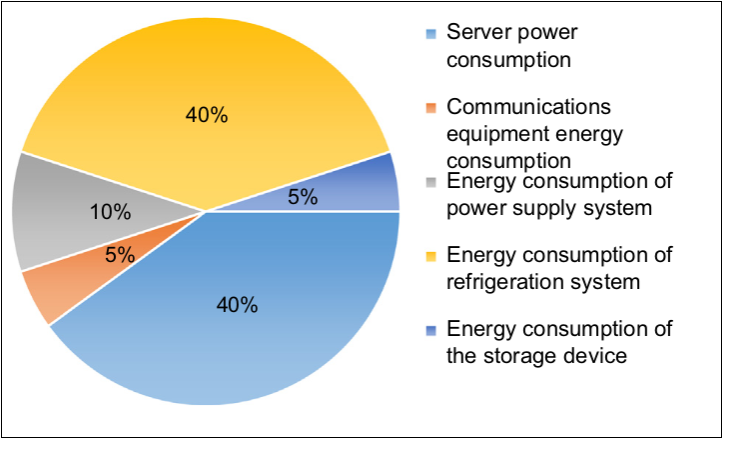
\includegraphics[width=0.5\textwidth]{pics/energyConsumption.png}
	\caption{Energy consumption distribution of data centers \cite{Rong:2016js}}
	\label{fig:consumption}
\end{figure}

Virtualization \cite{Uhlig:2005do} partitions a physical machine's resources (e.g. CPU, memory and disk) into several isolated unit called virtual machines (VMs) where each VM allows an operating system running on them. It rooted back in the 1960s' and was invented to enable isolated software testing. Soon, people realized it can be a way to improve the utilization of hardware resources. Thereafter, a resource management strategy of server consolidation was invented.

Server consolidation \cite{Zhang:2010vo} resolves the low utilization problem by gathering virtual machines (VMs) into a fewer number of physical machines (PMs), so that the resource utilization of PMs are maintained at a high level.  
In the meanwhile, idle servers are turned off to save energy.

\textcolor{Blue}{Difficulties}\\
Despite the usefulness of server consolidation, it is a difficult task. 
Server consolidation is often considered as a global optimization problem 
where its goal is to minimize the energy consumption. 
From mathematical model's point of view, it is often modeled as a bin-packing problem \cite{Mann:2015ua}.
Bin-packing problem is a well-known NP-hard problem meaning it is unlikely to find an optimal solution 
of a large problem. Previous research have studied the problem extensively. 
Because of its NP-hard nature, deterministic methods such as  
Integer Linear Programming \cite{Speitkamp:2010ck} and Mixed
Integer Programming \cite{Wang:2016eh} are unsuitable for a large scale problem 
because of the long computation time.  More research proposed heuristic methods
 to approximate the optimal solution such as 
First Fit Decreasing (FFD) \cite{Panigrahy:2011wk}, Best Fit Decreasing (BFD) \cite{Xu:2010vh}.
In addition, manually designed heuristics are designed to tackle the special requirements such 
as \cite{Li:2009wf, Gupta:2008ul, Jung:2008vb}. Although these greedy-based heuristics can quickly solve the consolidation problem,  As Mann's research \cite{Mann:2015ua} shown, 
server consolidation is a lot more harder than bin-packing problem - because of multi-dimension, many constraints - 
therefore, these greedy-based heuristics can not reach a good approximation and be easy to 
stuck at a local optima.

\textcolor{Blue}{New technology}\\
In addition, virtualization technology has evolved to allow finer granularity resource scheduling.
A recent advent of Container technique \cite{Soltesz:2007cu} has drove the attention of both industrial and academia.
Container is an operating system level of virtualization which means containers share the kernel within a VM and provide isolated environment for applications.
This new concept starts a new service model called Container as a Service (CaaS) \cite{Piraghaj:2015uf} is derived from Platform as a Service (PaaS). 
In comparison with traditional models, CaaS gives the responsibility of application 
deployment and resource allocation to the same hand of Cloud provider.
Hence, Cloud providers have a better control of their resources, however the management difficulty also increases. 
Currently, vast amount of research focus on VM-based server consolidaton can not be directly used on Contained-based model.
This thesis, therefore, aims at providing an end-to-end solution the contained-based server consolidation problem.


% World Energy Outlook 2013 \cite{energyOutlook} estimated world electricity demand for 
% data centers was expected to increase by 66\% over the 2011 to 2035. 
% Beyond that, data centers also have an enormous impact on carbon 
% dioxide emissions \cite{2010arXiv1006.0308B}.


% % A well-accepted measurement: PUE (Power Usage Effectiveness) \cite{Belady:IMLoaM62}
% % a standard measurement for data center energy efficiency which compares the 
% % total power with the power used to power IT equipment (e.g. server, network equipments). 
% A recent survey \cite{Cho:2016kz} shows that the recent development of cooling techniques 
% have reduced its energy consumption and now 
% server consumption has become the dominate energy consumption component.
% Despite improvements in hardwares, various software techniques have been proposed 
% to reduce the energy consumption of servers 
% such as: Server Consolidation and Dynamic Voltage and Frequency Scaling (DVFS) \cite{}.

% Virtualization \cite{Uhlig:2005ub} is the core technology that not only enables 
% the elastic management of Cloud resource but also can be used to improve the utilization and reduce 
% energy consumption.
% It maps a physical machine's system resource - including processors, memory, and 
% other devices - into isolated units called \emph{Virtual Machines (VMs)} which allows 
% multiple operating system to run on. 
% In essence, virtualization add an extra layer of software called 
% \emph{Virtual Machine Monitor (VMM)} or \emph{hypervisors} that can deploy, 
% release and migrate VMs at runtime. 
% Numerous VMMs have been designed for x86 commodity machines such as 
% Xen \cite{Barham:2003vu}, KVM \cite{Kivity:2007wu}, and VMware ESX server \cite{Barham:2003vu}.
 
% \textcolor{Maroon}{A brief introduction of server consolidation}

% It aims at improving the income by guaranteeing \emph{Quality of Service (QoS)}
% \cite{Calheiros:2011ul} of the maximum number of applications that a datacenter can accommodate.

% The server consolidation techniques on the server-level
% have been extensively studied in the past decade \cite{}. 
% However, the recent development of container technology enables a VM-level of consolidation, which 
% has not driven much attention. 
% Container is a lightweight virtualization
% technology which allows an application running in a single container. 
% Multiple containers can be packed in a single virtual machine. 
% Two main advantages make the container popular. 
% First, containers do not need a Virtual Machine Monitor (VMM) but relies on the operating system; 
% it reduces the overhead used on managing the virtual system. 
% Second, the communication \cite{} between containers are much 
% easier (e.g. inter-process communication) than an inter-VM communication. This feature is 
% particularly useful for micro-service-based Web applications where their processes are packed
% into separated containers.
% This new technology has brought new challenges to server consolidation. 
% Traditional algorithms can not be directly applied since there is an extra level
% of virtualization. Affinity and communication aware allocation play an much important role 
% in container-based environment. Therefore, new techniques and algorithms are need to be proposed. 

% Currently, few literatures address the 

% Therefore, this thesis will focus on providing solutions to 
% container-based server consolidation.

% Mainly, there are two types of method: static and dynamic.
% Static methods are often treated as off-line approaches and applied in a periodical manner 
% where a batch of VMs are allocated to a set of servers. 
% They are conducted at a given point of time when
% the overall utilization in a data-center is degraded into a certain level: 
% e.g, a predefined CPU utilization threshold. Because static methods often consider partial or all VMs
% in a datacenter, it is often treated as a global optimization task \cite{}.
% The static method often models the problem as a off-line bin-packing problem and 
% solved with deterministic or heuristic algorithms. The goal is often to find a global optimal solution
% in terms of server utilization and other criteria.
% Dynamic method is an on-line approach. It assumes a scenario when a single server is 
% overloading with multiple VMs, migrate one of the internal VMs out from 
% the host will release the overloading. Dynamic method is used in between 
% two static consolidation processes to ease the overloaded server as well as consolidation.
% As it only moves one VM at a time, it often applies greedy-based heuristic, therefore, hard to 
% reach a global optimization.





% This thesis, therefore, aims at
% providing an end-to-end solution to the container-based server consolidation problem.

% First, aggressive consolidation causes overloading physical resources. 
% It leads to performance degradation since the application cannot obtain enough resources
% the VM promised. It is hard to determine the maximum level of utilization of a physical machine.

\section{Motivation}
\label{sec:motivation}
\bx{This section identifies the research gaps in  resource management of container-based data centers.}
We will discuss the gaps from three placement decision scenarios: application initial placement, periodic optimization, and dynamic placement.

\subsection{Application initial placement}
\bx{Application initial placement deploys applications when data centers receive a number of requests.} The placement can be seen as a static server consolidation problem. To reduce energy, the strategy allocates applications to a minimum number of physical machines (PMs). For VM-based and container-based cloud, the energy models are different.
% The optimization process can be described as: given a number of  PMs represented as resources (e.g CPU cores and RAM etc);  requested applications (wrapped with VMs or container) represented as aforementioned resources; the objective is to allocate these applications into a minimum number of PMs. The decision variable is the location of each application. The basic constraint is that the aggregative resources of hosted VMs cannot exceed the PM's resource capacity.
% The strategies in VM-based cloud and container-based cloud are different. In VM-based cloud, requested applications (wrapped with VMs) are placed into a minimum number of PMs. The problem in VM-based cloud is often modeled as a bin packing problem \cite{Xiong:2014jq}, with VMs represent items and PMs represent bins. The complexity is NP-hard \cite{Hochbaum:1996ts}. 
\bx{In a VM-base Cloud}, the energy model of application initial placement can be seen as a vector bin packing problem \cite{Leinberger:1999fs}, applications (wrapped with VMs) are packed in PMs (detailed discussion is in Section \ref{sec:vector_bin_packing}).

\bx{In contrast, in a container-based Cloud, the energy model can be seen as a bilevel optimization problem \cite{Colson:2007bu} where each level is treated as a bin packing problem.} The lower level optimizes the placement of containers to VMs and the upper level optimizes the placement of VMs to PMs. The advantage the bilevel model is that the interaction of container-VM and VM-PM placement is considered, so that the global optimal can be achieved.

\bx{Two reasons motivate us to solve the application initial placement in container-based Cloud.} 
First, currently, no research has considered the application initial placement as a bilevel optimization problem. Therefore, it needs to propose a new bilevel energy model. A bilevel model - includes energy model, workload model and prices model - represents the relationship between container, VMs, and energy consumption. Current VM-based models cannot be directly applied because container-based model has two levels of placement. In addition, current VM-based models do not consider the overhead of VM hypervisor because for VM-based cloud there is no better ways to avoid the overhead. However, in container-based cloud, the overhead of VMs can be mitigated by reducing the number of VMs. This can be achieved by consolidating containers to fewer VMs. Furthermore, many VM-based models do not consider a balance between CPUs and memories. The balance is crucial \cite{Tomas:2013iv} in improving utilization of PMs, because the balance in a PM increases the probability of being able to allocating a new application.

\bx{Second, bilevel optimization is known to be strongly NP-hard \cite{Sinha:2013tn}.} Even in the simplest case of linear  bilevel programs, where the lower level problem has a unique optimal solution for all the parameters, it is not likely to find a polynomial algorithm that can find the global optimum solution. The proof for the non-existence of a polynomial time algorithm for linear bilevel problems can be found in \cite{Deng:1998fk}. In contrast, evolutionary computation (EC) is a population-based search mechanism which has been proposed to solve bilevel optimization problems \cite{Wang:2008kb, Wang:2011di, Angelo:2013ee}. EC algorithms have shown promising performance bilevel problems. Therefore, we will investigate EC-based approaches on bilevel problem.

% The optimization interact with VMs and containers, therefore, it cannot be optimized separately. An additional constraint is that each container has its OS requirement which makes them cannot be simply packed into homogeneous VMs. 

% \bx{Container-based placement can be seen as a bilevel optimization problem \cite{Colson:2007bu} where each level is bin packing problem.} Because of the problem structure has changed, previous VM-based approaches cannot be directly applied on the problem. In addition, currently, there is no study considers the container-based placement as a bilevel problem. The advantage of considering it as a bilevel problem is that containers and VMs can cooperate to achieve lower energy consumption. However, the \emph{optimization of joint placement of container and VMs} is very difficult because of the nature of bilevel problem.

% The hierarchy of bilevel optimization makes problems non-convex and strongly NP-hard \cite{Vicente:1994ie}.
% The placement problem in the VM context has been studied for years \cite{Xu:2010vh, Gao:2013gg, Ferdaus:2014ep} and it is often modeled as a bin packing problem . This is because VMs and PMs are naturally modeled as items and bins. Furthermore, server consolidation and bin-packing have the same optimization objective: minimize the number of bins/PMs. The complexity of bin-packing problem is NP-hard which is NP-hard \cite{Hochbaum:1996ts} which means it is extreme time-consuming to find its optimal solution when the number of decision variables is large. However, most research focus on VM-based server consolidation and these methods cannot be directly applied on container-based consolidation because of the different structure.

% \bx{Only few research focus on container-based server consolidation problem. One of research is from Piraghaj and et al \cite{Piraghaj:2015uf}.} They propose a simple heuristics on two-step allocation, thus, did not consider the interaction between two levels (see detailed discussion in Section \ref{container-based-placement}). 
% In addition, their resource allocation system completely relies on dynamic placement without using static methods. Although their system can execute allocation fast, the energy efficiency cannot be guaranteed. 
% Another research \cite{Mann:2016hx} is the earliest study which realizes two-level of placement should be considered together because they are interact with each other. They apply a fixed VM placement algorithm and considering a series of VM selection algorithms. The results also proves that the interaction between two placement cannot be ignored. 


\subsection{Periodic optimization}



% For the lower level of allocation, the objective is to maximize the utilization of resources (e.g a balanced utilization among several resources), while the upper level objective is to minimize the number of PMs. 
\bx{After initial placement, periodic optimization is a routine process that takes existing applications' placement, re-placing them to PMs to optimize the energy consumption.} A technology called live migration can be used to re-place the applications' placement from one PM to another. Live migrations are very expensive since they consume network bandwidth and use the resources on both host PM and targeted PM. Therefore, periodic optimization is a multi-objective task which considers minimizing migration of applications and minimizing the overall energy consumption. Resolving the bi-level multi-objective problem will lead to a high utilization of PMs but it is very challenging.

\bx{Two reasons motivate us to explore solutions for periodic optimization in a container-based cloud}. 
\textbf{First}, no research has considered the periodic optimization in a container-based cloud as a bilevel multi-objective optimization problem. The multi-objective bilevel problem has two potentially conflicting objectives: reducing the number of migration and minimizing the energy consumption.
\textbf{Second}, not many research have considered the robustness of placement. The robustness of placement means the placement is resilient enough to handle the fluctuate workloads without making too many further adjustments. To achieve robustness of placement, periodic optimization must consider the combination of various workloads and the reserved resources on PMs. Currently, most research simplified workloads as static (remains a constant value throughout its life cycle) \cite{Viswanathan:2012ej, Chen:2011fl,Feller:2011vs} for the sake of simplicity. The placement is easy to affect by fluctuations which leads to higher energy consumption. Therefore, we will consider various types of workload to improve the robustness of placement.
% For example, for periodic workload, the average value within a period of time will be considered. 

% \bx{In our research, we will consider periodic optimization as a multi-objective problem with various types of workload \cite{Fehling:2014tl}.} Specifically, complementary workloads can be combined so that it can potentially reduce the migration in the future. Thus, the applications are consolidated in a more robust way. 

% However, in real life, workloads vary with time. According to Fehling , applications' workload are roughly classified into five categories: static, periodic, once-in-a-life-time, continuously changing, and unpredictable. 

% They cannot be treated as a static value in a server consolidation because Therefore, it increases the cost in the future. 




% Only a few research consider applying different strategies on different workloads \cite{Meng:2010gh}. Their experiments showed promising results, however, they only mapped paired workloads which can be further improved by combining multiple workloads.
\subsection{Dynamic placement}


\bx{Dynamic placement is applied on overloading and underloading scenarios which need an immediate reaction on the placement of an application \cite{Beloglazov:2013ht}.} Overloadding and underloading happened when applications are released from PMs or applications are facing a burst of workload. In overloading scenario, PMs are running out of resources which means the applications' performance degraded. The degradation will bring financial punishment for Cloud providers. In underloading scenario, PMs are running in a low utilization which leads to the waste of energy. At these states, it is ideal that applications inside the PM will be placed to other PMs to quickly resolve the problems.
% Overloading is a scenario that the workloads exceed the capacity of its host PM. Hence, one or more applications will be migrated to other PMs. Underloading is when a PM runs in a low utilization, all the applications inside it will be moved to other PMs, so that the PM can be turned off. The common operation in these two scenarios are the dynamic placement \cite{Xiao:2015ik}. Dynamic placement places one application each time in an on-line manner. 

\bx{Three reasons motivates us to explore solutions for dynamic placement}. 
\textbf{Firstly}, no research has considered dynamic placement in container-based cloud as a bilevel problem. Current approaches \cite{Piraghaj:2016bw} consider two placements as separate tasks. 
\textbf{Secondly}, current VM-based dynamic placement approaches typically applied either simple bin-packing algorithms such as First Fit or manually designed heuristics. Simple bin-packing algorithms may perform poorly because application placement is more complicated than bin-packing \cite{Mann:2015ua}. Therefore, even for the placement of VMs to PM, it is difficult to reach a global optimal solution. \textbf{Thirdly}, manually designed heuristics may not be general (in terms of decision variables and constraints) because they are designed for specific conditions and constraints \cite{Jung:2010dt}, e.g considered the network topology in data centers. We want to develop a hyper-heuristic approach which can automatically generate good heuristics based the knowledge learned from previous placement solutions.

% The hyper-heuristic can learn from previous good solutions as well as the features of various workloads so that the dispatching rules can be applied with any conditions and constraints. 
% on one hand, dynamic placement allocates an application at a time to meet the requirement of fast reaction. On the other hand, it only considers the best placement of the current application using either simple bin-packing algorithms such as First Fit or manually design heuristics. Simple bin-packing algorithms may perform poorly because application placement is more complicated than bin-packing \cite{Mann:2015ua}, while manual designed heuristics may not be general because they are designed for specific conditions and constraints\cite{Jung:2010dt}.
% Mann's research  showed, server consolidation is a lot harder than bin-packing problem because of the multi-dimensional of resources, heterogeneous PMs, migration cost etc. 


In summary, shortcomings of current resource management in container-based cloud increase the energy consumption of a cloud data center. Therefore, our goal is to reduce the energy consumption by overcoming these limitations in each of placement decision scenario.


% \bx{These challenges motivate us to develop a hyper-heuristic approach which can automatically generate heuristics for quickly placing.} 

% In addition, in container-based Cloud, the placement target is on containers and the destination is a suitable VM. However, if no VM can accommodate a container, a new VM must be created, which incurs a second level of deployment.

% \bx{In summary, this thesis aims at improving the energy efficiency in a container-based cloud data center.} The gaps in three resource management processes motivate us to address three issues:
% \begin{itemize}
% 	\item Develop an algorithm for the joint placement of containers and VMs.
% 	\item Develop an algorithm for multi-objective joint placement of containers and VMs with consider various workloads.
% 	\item Develop a hyper-heuristic for dynamic placement.
% \end{itemize}




% The motivation for this thesis mainly includes two parts, in the first part, we illustrate the roots of container-based server consolidation problem. In the second parts, we explain the motivations for the objectives.

% \subsection{Motivation For Container-based Server Consolidation Problem}

% Server consolidation \cite{Zhang:2010vo} resolves the low utilization problem by gathering applications or VMs into a fewer number of physical machines (PMs), so that the resource utilization of PMs are maintained at a high level. In the meanwhile, idle servers are turned off to save energy. Traditional server consolidation is VM-based, in comparison with 
% a server host a single application, it can dramatically improve the resource utilization. 


% \begin{figure}
% 	\centering
% 	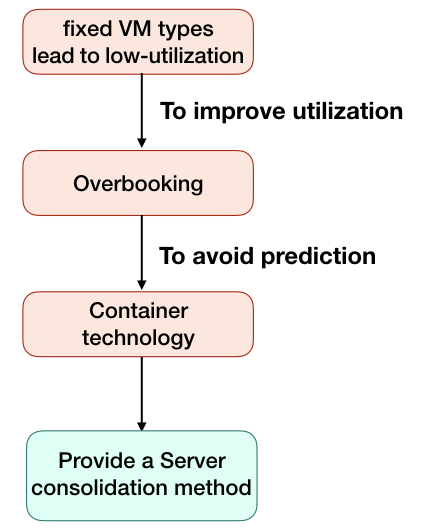
\includegraphics[width=0.3\textwidth]{pics/problem_flow.png}
% 	\caption{The root of container technology}
% 	\label{fig:root}
% \end{figure}
% \begin{enumerate}
% \item Container is a new virtualization technology which provides an operating level of virtualization.
% % Figure \ref{fig:root} illustrates the root of container technology from an energy efficient point of view. 

% In order to solve this problem, overbooking strategy tends to place more VMs than the server's maximum capacity. However, this technique is highly relied on workload prediction on the application running in a VM. Otherwise, servers are easily overloaded. Container technique can improve the utilization by further partitioning VM into resource isolated chunks. Therefore, multiple applications can share the same VM. This technique avoids the prediction of workload as well as improving the utilization. 



% This container technology brings many advantages to current Cloud industry\cite{Felter:2015ki}but it also brings difficulties for server consolidation. Container-based server consolidation adds another level of abstraction which makes it a two-level vector bin-packing problem.
% Therefore, it motivates us to provide \emph{global optimized} resource allocation solution for container-based data centers.

% \end{enumerate}


% \subsection{Motivation For Research objectives}
% Cloud data center has a high dynamic nature where it constrantly receives new requests for resource provisioning and releases old current resources. Therefore, a data center needs different strategies to
% handle different scenarios. 

% \textcolor{Maroon}{In this thesis, we aim at providing a series of approaches to continuously optimize the joint allocation of VMs and containers which involves with three scenarios: application initial placement, periodic consolidation, and dynamic consolidation.} Different stages have distinct goals, therefore, they are considered as separated research questions. 

% \begin{enumerate}
% \item Joint allocation of containers and VMs (application initial placement), \\
% \textcolor{Maroon}{Joint allocation of containers and VMs is the first task when a data center receives new application deployment requests.} At this stage, a set of containers is allocated to a set of VMs and these VMs are allocated to a set of PMs. This task is challenging because the problem is a bilevel optimization where each level is a bin packing problem. Exhaustive search of entire solution space is practically impossible, for the number of possible permutation of solution is huge. Current approaches \cite{Piraghaj:2016bw,Hindman:2011ux} use simple heuristics such as First Fit to solve the problem. These greedy-based heuristics do not consider the complex structure of the problem, therefore, often reach a local optimal solution.

% Only a few research focus on this  problem, Piraghaj \cite{Piraghaj:2016bw} designs a dynamic allocation system. She proposes a two-step procedure. Since, these two-level structure interact each other, separate solution certainly leads to a local optima. Therefore, in this thesis, we will solve the problem simutaneously.
% Most importantly, and therefore can not be solved separately. This is the first research that consider server consolidation has a bi-level optimization problem \cite{Wen:1991kt}. 

% In this objective, we will establish the fundamental concepts in studying this joint allocation of containers and VMs including new problem models: price and power model, new problem constraints, and optimization objectives. The major challenges for this objective is to design representations and several EC approaches to solve this problem. More specifically, in designing the EC approach, new search mechanisms, operators will be designed and new representations will be proposed to fit the problem. 

% This task is challenging, since a representation can highly affect the performance of consolidation \cite{SoteloFigueroa:2013be}. 

% \item Periodic consolidation, \\
% \textcolor{Maroon}{A periodic consolidation is conducted to improve the global energy efficiency in a periodical fashion.} Data center constantly receives new allocations, releasing of old resources. These changing degrades the compact structure of a data center. Therefore, the data center needs a global optimization to improve the overall energy efficiency.

% The challenges are three folds, firstly, similar with initialization problem, the problem has two level of allocations and they interact with each other. Secondly, like VM-based consolidation, Container-based consolidation is considered as a multi-objective problem with minimization of migration cost as well as keeping a good energy efficiency. In bilevel optimization, multi-objective can be defined in either or both level, therefore, it further increases the complexity. Thirdly, consolidation needs to consider different types of workload which may lead to more migrations in the future(\textcolor{Maroon}{NEED MORE EXPLANATION}).

% \item Dynamic consolidation,\\
% Dynamic It takes one container and allocates it to VMs. Since the size of container can be dynamically adjusted, when the an application is under-provision or over-provision, the original container is halted, resized and re-allocated. Hence, there is a need to allocate this new container in real time.

% To solve a dynamic consolidation, heuristics and dispatching rules are often used \cite{Sarin:2011fu, Shi:2011ke, Forsman:2015ca, Beloglazov:2012ji}.  In this scenario, a dispatching rule is considered as a function that determines the priorities of VMs that a container can be placed. However, dynamic placement is much complex than bin-packing problem \cite{Mann:2015ua}. Because of its dynamic nature, human designed heuristics are ill-equipped in approximating solutions when the environment has changed \cite{SoteloFigueroa:2013be}. 

% Hyper-heuristic methods, sepcifically, Genetic Programming (GP) technique \cite{Banzhaf:1998wc} can learn from the best previous allocation and automatically evolves dispatching rules to solve this problem. GP has been applied in generating dispatching rules for bin-packing problem \cite{Burke:2006ei, SoteloFigueroa:2013be} and other scheduling problems \cite{Nguyen:2014eu}. The results have shown promising results.

% There are mainly two challenges, first, it is difficult to identify the related factors that construct the heuristic. Factors or features are the building blocks of heuristics. It is a difficult task because the relationship between a good heuristic and features are not obvious. Second, representations provide different patterns to construct dispatching rules. It is also unclear what representation is the most suitable for the consolidation problem.


% and representations must be proposed to capture the characteristic of the joint allocation. 
% 	and the VMs are allocated to physical machines in the second step. Because of the complexity, previous research
% 	only considers the first step. They map the incoming tasks into predefined categories and based on the characteristic of the categories, the size of new virtual machines' resources are decided. After each tasks have chosen its VM type, they are allocated to virtual machines using a lightweight heursitic algorithm. 
% 	We intend to apply an EC-based approach to solve this problem by proposing a coevolutionary that simuetiously decide the virtual machine type as well as the allocation of VMs.


% \item Large-scale of static server consolidation problem, \\
	% In this case, initialization and periodic consolidation are belonged to this category. 
	% Since Cloud data center typically has hundreds of thousands PMs and more, static server consolidation is always very challenging. Many approaches have been proposed in the literature to resolve the problem. There are mainly two ways, both relied on distributed methods, hierarchical-based \cite{Jung:2010dt, Moens:2011gk} and agent-based management systems \cite{Yazir:2010bk}.
	% The major problem in agent-based systems is that agents rely on heavy communication to maintain a high-level utilization. Therefore, it causes heavy load in the networking. 
	% Hierarchical-based approaches are the predominate methods. In essence, these approaches are centralized methods where all the states of PMs within its region are collected and analyzed. The major disadvantage of hierarchical-based approaches is that it only provides local solutions. In fact, it is infeasible and unnecessary to check all the states of PMs since the search space is too large and most PMs do not need a change. This idea
	% motivates a way to improving the effectiveness is to reduce the number of variables so that the search space is narrowed. In this thesis, we are going to investigate the way to eliminate the redundant information.
% \end{enumerate}



% Traditional Cloud computing offers three services models: Infrastructure as a Service (IaaS), Platform as a Service (PaaS) and Software as a Service (SaaS). Both IaaS and PaaS describe how does a service provider use the cloud resources. The main difference of these two models are  
% IaaS allows service providers to manage the low-level details including the operating system and libraries. While, PaaS provides a higher level of abstraction where users only focus on the application development without caring the underlying operating system and system-level of resources such as CPU cores and memories. However, one drawback of PaaS is that cloud users must make sure their applications are complete compatible with the platform. And in many of the cases, it is not the situation. In order to solve this problem, a container-based virtualization technology starts to reform the Cloud industry. Container as a Service (CaaS) 
% is a new concept but it has been used in industry for many years. Containers provide an operating system-level of isolation environment for applications. It does not need a hypervisor but complete rely on the operating system. 


% This exciting new technology has bring so many advantages for both Cloud users and Cloud providers. From the providers' perspective, In a large system, running VMs means there are probably many same operating systems occupying memories and storages. Lightweight containers share operating system and therefore, there are more rooms for softwares. It increases the capability of Cloud data centers. Furthermore, in terms of resource utilization, it provides much finer granularity operation than a VM-based Cloud model. Containers partition
% a VM into smaller chunks so that with appropriate management, better energy efficiency can be achieved. From the cloud users' perspective, each container provides separated libraries for specific application.  Therefore, it does not contrained by the underlying platform. Like PaaS, Cloud users do not need to concern the scalability of applications. 
% Therefore, CaaS can potentially become one of the main stream in the future Cloud computing industry. 

% Secondly, energy-efficent computing has been the major concern since the begining of computers. Specifially, Cloud computing has become a popular form. Large-scale data centers have been built around the world. A data center can consume huge amount of energies and it needs to improve its energy-efficiency from multiple perspectives. As we discussed in the Introduction, computing servers are one of the major contribution to the energy consumption. 
% And according to observation by \cite{}, the average utilization resource are still very low which causes huge energy wastage. As we mentioned above, the container technolgy provides a better way of managing resources, it has the potential to largly improve the utilization than current VM-based Cloud model because it avoids some of the major drawbacks of VM-based model. 

% Thirdly, because the container technology is relatively new, previous research are mostly focus on IaaS model and so that the server consolidation has based on the VM-level. However,   

% Frist is this new technology of container that can potentially change the landscape of
% Cloud computing. It has so many benefits but also it brings difficulty in managing resources.

% Second, from green computing point of view, we still need to manage resource so that, the 
% data centers consume less energy. And container technolgy actually bring a better chance to
% be more energy-efficient than previous VM based technology.
% Third, it is very difficult to manage this container-based resources because of the problem-nature is too complicated. And existed algorithms can not be directly applied on it.
% Fourth, the evolutioanry computation provides a good framework to handle such difficult problem.

% \textcolor{Blue}{Motivation is what is now lack from the literature.} \\

% The advantage of Platform as a Service (PaaS) has been discovered in the recent years. 
% The disadvantage of tranditional IaaS model has been discovered in the recent years \cite{Mann:2016hx}.
% In IaaS, on one hand, cloud customers need to manage the low-level details ranging from application capacity estimation,
% resource planning and selection and deployment. 
% On the other hand, Cloud providers manage resource provisioning and allocation. 
% Although these two tasks are seemingly different, 


% The container as a Service (CaaS) cloud model has gain increasing attention in the recent years.
% However, the energy efficiency in CaaS cloud environment has not been investigate. 
% Particularly, the virtual machine and container joint consolidation is the core problem.
% Therefore, in this thesis, we will focus on the end-to-end energy-aware server consolidation on container-based
% Cloud. In the meanwhile,  a major research direction of large scale server consolidation is also considered. 
% The end-to-end server consolidation refers to the server consolidation techniques used
% in the different stages throughout the routine Cloud resource management including  initial VM provisioning and placement, dynamic VM placement, and static VM placement:

\section{Research Goals}

\begin{figure}
	\centering
	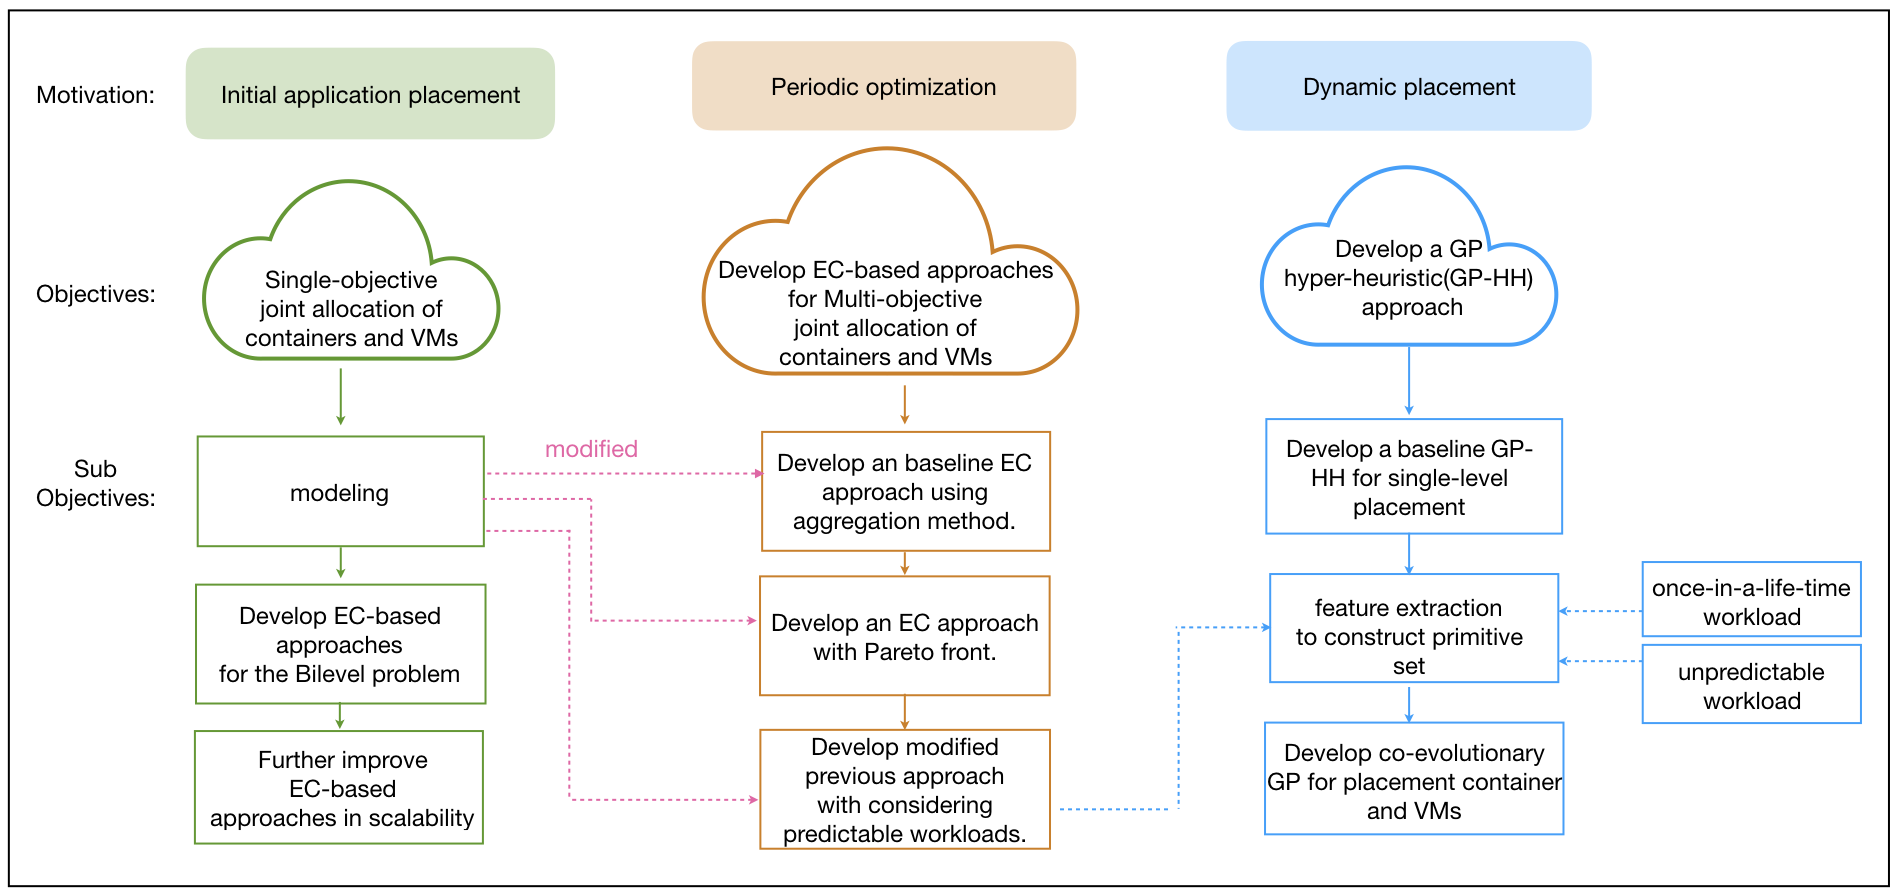
\includegraphics[width=\textwidth]{pics/thesisPlan.png}
	\caption{Relationship between objectives}
	\label{fig:objectives}
\end{figure}
\bx{The overall goal of this research is to optimize energy consumption of a container-based Cloud data center using EC-based approaches for three placement decision scenarios:} initial placement of application, periodic placement of application, and dynamic placement of application. The specific research objectives of this work can be itemized as follows.
% In this thesis, we aims at providing a series of approaches to continuously optimize the a joint allocation of VMs and containers that considers three consolidation scenarios: Initialization, global consolidation, Dynamic consolidation. In addition, the static allocation normally involves with large amount of variables which is particular difficult to optimize. We are also going to propose a method to solve this problem.  These approaches combine element of AI planning, to ensure the objectives and constraint fulfillment, and of Evolutionary Computation, to evolve a population of near-optimal solutions. The research aims at determining a flexible way in creation of solutions to solve server consolidation problems. As discussed in the previous section, the research goal can be achieved in the following objectives and sub-objectives.

\subsection{Objective One: Develop EC-based approaches for the single objective joint placement of containers and VMs for initial placement of application}
\label{sec:obj1}

\bx{The goal of objective one is to minimize energy consumption in initial placement of application at container-based cloud.} We set three sub objectives to achieve this goal. The first sub objective is to propose a new bilevel energy model for the joint placement of containers and VMs in PMs. The second sub objective is to develop an EC-based optimization algorithm to solve the joint placement of containers and VMs. The third sub objective improves scalability of the proposed EC-based optimization algorithm. Note that, we will use ``the bilevel model/problem'' to replace ``the joint placement of containers and VMs model/problem'' in the following content. 
% \textcolor{Maroon}{Currently, most research on container consolidation do not consider the two-level of allocation problem.} Unlike previous VM-based service consolidation, 
% most research focus on VM-based server consolidation technique. They often modeled the VM allocation problem as a vector bin-packing problem \cite{Zhang:2016cx}. 
% Container adds an extra layer of abstraction on top of VM. The placement problem has become a two-step procedure, in the first step, containers are packed into VMs and then VMs are consolidated into physical machines. These two steps are inter-related to each other. Previous research \cite{Piraghaj:2015uf} solve this problem in separated steps where the first step allocates containers to VMs and the second step allocates VMs to PMs with simple bin-packing heuristics. According to Mann's \cite{Mann:2016hx} observation, these two allocations should be conducted simultaneously to reach a near-optima solution, which essentially minimizes the energy consumption.

\begin{enumerate}
	\item Develop a new bilevel energy model to represent the relationship between six factors and energy consumption. The five factors involves locations of container, types of VM, locations of VM, overheads of VM, and the balance between memory and CPU. We need to consider the interaction between these factors.
	% \textcolor{Maroon}{This problem can be considered as a bilevel problem \cite{} the lower-level optimization: allocate containers to VMs and the upper-level: allocate VMs to PMs.} 
	% \textcolor{Maroon}{Since the existing models for container-based consolidation are based on VM-based model which incurs two problems.}
	% First problem is that they did not consider the interaction between two levels of allocation.
	% Second problem is that they did not consider balancing the residual resources (e.g between CPU and memory). 
	% \bx{The goal of the first sub objective is to propose a bilevel model for the joint placement of container and VM.} 

	\bx{The major challenge of this sub-objective is that the bilevel energy model is more complicated than a single-level energy model.}
	\textbf{First}, in VM-based model, the only factor is the locations of VMs in PMs. In contrast, in container-based model,  the energy model involves with four more variables such as the locations of containers in VMs, types of VM, overheads of VM, and the balance between memory and CPU. Specifically, the factor of locations of container decides the placement of applications. We consider types of VM because the containers may have constraints on the types of VM. Overheads of VM should also be considered because appropriate placement containers can minimize the overheads of VM. The balance of CPU and memory has an impact on the energy consumption \cite{Mishra:2011bz}. The better balance will lead to a higher probability of being able to allocate more applications.

	Three challenges are listed as follows. \textbf{First}, the bilevel energy model is more complicated than a single-level energy model. The relationship among variables of the bilevel energy model has not been explored. In the VM-based energy model, the only variable is the location of VMs in PMs. In contrast,  container-based energy model has more variables such as the location of container, type of VM and the location of VM. \textbf{Second}, the balance of CPU and memory has an impact on the energy consumption  The more balance between CPU and memory in a PM, the higher probability of being able to allocate more applications. However, in container-based cloud, defining this balance is not straightforward because an additional variable of VM type has not been considered in previous study. \textbf{Third}, the overheads of VMs has not been considered in VM-based model because there is no better way to avoid the overheads. However, in container-based cloud, the overhead of VM can be mitigated by reducing the number of VMs. Therefore, adding the overhead of VM to the container-based energy model is necessary. 

	% The first issue is that it is still unclear that which energy function is the best to capture the relationship between container and VM so that the overall energy is low. Specifically, the objective for the lower level - placing container to VM, is still unclear. This is because the minimum number of VM does not necessary lead to the minimum number PMs; the types of VM also play an important role.
	% The second issue is that previous VM-based research do not consider the overhead of VM. However, the overhead of VMs is a major source of resource wastage (addressed in Section \ref{sec:comparison_container_vm}). Therefore, how to represent the impact of VMs remains unsolved.
	% The third issue is related to a VM-based research,  Mishra \cite{Mishra:2011bz} discovered that when multiple resources are considered in the model, the balance between resources has a heavy impact on the optimization results. Therefore, in the bilevel model, the balance of resources should also be considered.

	In order to establish a bilevel energy model, we will follow three steps. First, we will review a number of literature discussing the overheads of VMs. One possible way is to represent the overheads of VMs as the utilization of resources. The relationship between the utilization of resources and the types of VM needs to be investigated.  Second, we will review literature about how to represent the balance between CPU and memory. For the bilevel energy model, both VM and PM requires a balance between CPU and memory so that the utilization can be maximized in both levels.

	the VM-based energy model to establish the variables and constraints. The relationship between VM, PM and energy consumption can be found in literature. However, the relationship between container and VM is not straightforward because of the overhead of VM and 

	Each level of the problem will be formulated to a multi-dimensional vector bin packing problem. 
	We will start from the simplest case - single dimension of resource - to more general multi-dimensional resources model by reviewing a number of VM-based approaches. Specifically, we focus on their variables, constraints and objective function. Objective function is mainly related to energy consumption. Hence, energy model is another major issue to study. In addition, in the multi-dimensional resource model, we will address the balance of CPU and memory problem by investigating several resource wastage models \cite{Ferdaus:2014ep, Xu:2010vh, Gao:2013gg}. In this objective, we consider the static workload of applications, this is because the initial resource demand is often provided by the Cloud users.


	% The novel contribution of this sub-objective is 


	\item Propose a new EC based bilevel optimization approach to solve the initial placement of application.\\
	\bx{Based on the proposed bilevel model, the goal of this sub-objective is to develop an approach for the bilevel optimization problem using nested Evolutionary algorithms \cite{Sinha:2017et}.}

	\bx{Three challenges need to be solved. First one is to understand the interaction between bilevel's placement.} In the bilevel problem, placing containers into a minimum number of VMs does not necessary lead to the minimum energy consumption. Therefore, it is still unclear that relation among the selection type of VM, placement of container and placement of VM will affect the energy consumption. Second challenge is how to design the search operators and representation. Currently two types of representation: direct and indirect representation can be considered. However, it is unclear that which one is more suitable for the nature of the bilevel problem. Third, bilevel optimization is strongly NP-hard \cite{Mathieu:2011dw}, the solution space can be non-linearity, discreteness, no-differentiability, and non-convexity. Therefore, it is extremely difficult to design a proper search mechanism to find near optimal solutions.

	In order to discover the relation among the selection type of VM, placement of container and placement of VM, we will first use one type of VMs and one type of container. By controlling these variables, the effect of different types of VMs and containers will be eliminated. Therefore, the relationship between bilevel placement would be clear. We will gradually add up variables and constraints. For the representation of bilevel problem, we will develop direct binary representation \cite{Xu:2010vh}, and indirect continuous probability representation \cite{Xiong:2014jq}. Genetic operators are also designed along with the proposed representation.
	Current nested methods have been used in solving bilevel problem, however, there is no research focus on bilevel bin-packing problem. We will investigate several approaches such as Nested Particle Swarm Optimization \cite{Li:2006br}, Differential evolution (DE) based approach \cite{Angelo:2013ee, Zhu:2006in} and Co-evolutionary approach \cite{Legillon:2012dd}.

	\item Investigate methods to improve the scalability of the EC-based bilevel optimization approach.

	\bx{Based on proposed EC-based approach, the goal of this sub-objective is to improve scalability of the approach.} Although nested approaches have been reported effective, they are very time consuming \cite{Sinha:2017et}. Therefore, this sub objective intends to explore other directions to improve the execution time. 

	\bx{Three approaches can be potentially used in improving the scalability.} The first one is single-level reduction \cite{Sinha:2017et}, which reduces the bilevel problem into a single dimensional problem. Containers can be categorized into VMs which is then placed into PMs. The combination of container must be based on the knowledge of two-level placement interaction which we discover in the previous objective. Clustering approaches such as K-means \cite{Xie:2011fj} or decision tree can be useful in categorizing containers. Then, complementary containers can be grouped to reduce the variables of placement. The challenge is to identify the features of static workload so that different workloads can be combined to fill a VM. Another way is use reinforcement learning to learn the pattern of energy-efficient combination of containers. 
	The second approach is using a divide and conquer method to split the large number of containers into smaller chunks. The main challenge is that how to split the problem is unknown. Randomly dividing is very likely lead to a sub-optimal solution.
	The third approach is combine heuristics into the EC algorithm, for example, develop a representation which is embedded with a simple heuristic (e.g First Fit). The heuristic is expected to reduce the search space so that the EC algorithm can find solution more efficiently. However, design a heuristic which embedded inside an EC algorithm is extreme difficult since evaluation of heuristic is indirect. 

	% \item Third, although nested approaches have been reported effective, they are often very time consuming. Therefore, our third sub-objective will focus on developing more efficient algorithms. There are several possible directions to be explored such as metamodeling-based methods \cite{Wang:2007em} and single-level reduction. 
		% \emph{New operators and searching mechanisms}\\
		% In order to utilize Evolutionary Computation (EC) to solve this problem, we are going to develop searching mechanisms according to the nature of problem as well as the selected representation. In order to achieve this goal, we will design several new operators. In order to evaluate the quality of these components, we will perform analytical analysis on the result.
\end{enumerate}
\subsection{Objective Two: Develop EC-based approaches for the multi-objective joint allocation problem for periodic placement of application}
The goal is to develop multi-objective EC-base approaches for container-based cloud in periodic placement of application with considering various types of workload to reduce the overall energy consumption.

% As previously (see Section  \ref{sec:motivation}) mentioned, the task is multi-objective: minimizing the number of migration and minimizing the overall energy consumption. This two objectives are conflicting since intensive optimization may incur a large number migration. The first challenge is how to solve the multi-objective bi-level optimization problem. In addition, we consider propose a robust periodic placement of application which means the placement of applications does not affect much from the variant workloads. Therefore, we divide workloads into five categories according to Fehling \cite{Fehling:2014tl}: static, periodic, once-in-a-life-time, continuously changing, and unpredictable. Among five types of workloads, two of them:  once-in-a-life-time and unpredictable workloads are unsuitable for static placement, since their behavior are hard to foresee and plan, hence, they are normally solved by dynamic approaches which will be addressed in our third objective.  For static, periodic, and continuously changing workload, we are going to design specific solutions. We also use three questions to guide our objective.
% The robustness of a data center is particularly important. 
% The robustness measures the stableness of result of consolidation.
% Furthermore, we will investigate proactive approaches - considering future allocation.
% In order to measure the degree of robustness, we need to design a robustness measure. The second sub-objective is to design static consolidation algorithm with considering its previous immediate result. The third objective extends the second objective to a more general case, considering both previous immediate and next allocation. The evaluation of algorithm is based on analytical analysis of fitness functions and robustness measure. 

\begin{enumerate}
	\item Modify the proposed model to adapt to the multi-objective problem with various types of workload. \\
	\bx{The goal of this sub-objective is to modify previous proposed bilevel model so that it adapts to the multi-objective problem.}

	\bx{There are mainly two challenges, the first one is to add an migration model to the existing model, and the second is to adapt the model to various types of workload.} The migration model is distinct with VM-based model. Because both container and VM can be migrated, it is unclear that migration model should be added to both layer or just one. One possible solution is to represent all VM migration with container migration. It may reduce the complexity. In addition, majority traditional migration models only consider the migration number without including the size of the applications which is unrealistic. Because the size will affect the overhead on the networking. 
	The second challenge is to adapt the model to various types of workload. Previously, we simply the problem as applications can be represented as static workloads. In this sub objective, we consider three types of predictable types of workload: static, linear continuous changing and periodic workload. These workloads may be represented as a function of time. Other models may also be changed accordingly.

	% We will further develop an EC-based multi-objective algorithm with aggregation approach to test the model. The aggregation approach turns a multi-objective problem into a single-objective problem by combining objectives into a single one. Therefore, we may use previous developed algorithm to solve periodic placement of application problem. We will use static workload to test the model. 

	\item Propose an EC-based multi-objective algorithm for periodic placement of application with Pareto front approach.\\
	\bx{The goal of this sub-objective is to develop an EC-based approach to solve the multi-objective joint allocation problem with Pareto front approach.} 

	The major challenge in this sub-objective is to design genetic operators so that the proposed algorithm can steer the search close to the correct Pareto front. The aggregation approach proposed in previous sub objective has some defects such as it cannot find the non-convex solution. A Pareto front approach is able to find a set of trade-off between objectives, therefore, we decide to explore this direction. Currently only a few research \cite{Yin:2000bt, Deb:2009jh,Deb:2010in} focus on bilevel optimization problem. This will be the first time that bilevel optimization with Pareto front approach is applied on a bilevel bin packing problem.
	% However, most of them are designed for continuous problems. Therefore, new representations and operators need to be considered for discrete problem. 

	% The assumptions for this objective, we will start from one dimensional of resource: CPU utilization. We will consider the static workload in this sub objective because they are common and easy to start with.  We can utilize the representation and problem models from previous objective. However, we need to propose new genetic operators to adapt the multi-objective problem.

	% like the case in single objective problem, we need to develop new representations, genetic operators.
	\item Propose an EC-based multi-objective algorithm for periodic placement of application considering various types of predictable workload. \\
	\bx{The goal of this sub objective is to propose an approach for three predictable workloads \cite{Fehling:2014tl}: static, linear continuously changing, and periodic.} The major challenge for this objective is that the change of problem model from static to changing workload may lead to a different representation. In order to achieve using a uniform representation for various workload, we are going to explore various workload. Accordingly, new search mechanisms must be proposed to adapt to the representation.
	% Factor analysis such Principle Component Analysis \cite{Wold:1987wx} can be employed in developing new measure. Meanwhile, the representation used in static workload might not work, therefore, new representation, genetic operators need to be developed. 

	% Proactive consolidation \cite{Farahnakian:2015vj, Tan:2011jd} has driven a lot of attention in recent years. They mainly focus on making prediction of the workloads using a regression approach such as linear regression, multi-linear regression, and K-means regression. However, most of their consolidation methods are simple heuristics. In our approach, we seek to propose a combined technique.

	% \item Second, we will design a robustness measure. Previous studies only use simple measurement which counts the migration number between two static consolidation. This measurement aims at minimizing the number of migration between two  static placement processes. It may cause more migration in the next consolidation. Therefore, it needs a time-aware measure of the robustness of system. Therefore, in this objective, the first sub-problem we are going to solve is to propose a robustness measure. Currently, only a few research propose robustness aware server consolidation techniques \cite{Takouna:2014fa, Grimes:2016ia} have been proposed. They are either static threshold or probability-based threshold to measure the robustness of PMs. We will investigate an adaptive measure based on the historical data and current status.
	

	
	% \item \emph{Design a }\\

		% We will generalize the previous sub-objective to a more general one: design a time-aware allocation method which takes previous and next allocation into consider.
	\end{enumerate}

\subsection{Objective Three: Develop a hyper-heuristic single-objective Cooperative Genetic Programming (GP) approach for automatically generating dispatching rules for dynamic placement of application.}

\bx{The goal for this objective is to develop a cooperative GP-based hyper-heuristic algorithm so that the generated dispatching rules can achieve both fast placement and global optimization with various workloads.}

% Previously, dynamic consolidation methods,including both VM-based and container-based, are mostly based on bin-packing algorithm such as First Fit Descending and human designed heuristics. As Mann's research \cite{Mann:2015ua} shown, server consolidation is more harder than bin-packing problem because of multi-dimensional of resources and many constraints. Therefore, general bin-packing algorithms do not perform well with many constraints and specific designed heuristics only perform well in very narrow scope. Genetic programming has been used in automatically generating dispatching rules in many areas such as job shop scheduling \cite{Nguyen:2014eu}. GP also has been successfully applied in bin-packing problems \cite{Burke:2006ei}. Therefore, we will investigate GP approaches for solving the dynamic consolidation problem. We will start from considering one-level of problem: migrate one VM each time to a PM. 

% Therefore, in this objective, we will use GP to automatically generate heuristics or dispatching rules.

\begin{enumerate}

	\item Develop a GP-based hyper-heuristic (GP-HH) algorithm for the placement of container to VM. \\
	\bx{In order to develop a cooperative GP-based hyper-heuristic to the bilevel problem, it is necessary to develop a GP-HH for the single level of the problem. Therefore, the goal of this sub-objective is to develop a GP-HH algorithm for placing containers to VMs.} This task is none trivial since no GP-HH has been dynamic placement of application problem. Therefore, we may start from considering the features such as the status of VMs (e.g resource utilization), features of workloads (e.g resource requirement) that will affect the placement decision. We will construct primitive set with the selected features. Other unsolved issues are the functional set and search mechanism. We will use the functional set by using the general operators. The original genetic programming will be used as the search mechanism. 

	To train the GP-based hyper-heuristic, we will use the solutions in the first objective as the model solution. 

	In order to evaluate the automatically generated heuristics. We will use a widely used simulator called CloudSim \cite{2009LNCS.5931...24B}. Since our proposed algorithm is focus on one level of placement, it is equivalent to the VM-based placement problem. We will compare our heuristic to a highly cited work \cite{Beloglazov:2012ji} from Beloglazov who propose a Best Fit Decreasing heuristic for the energy consumption problem.

	\item Conduct feature extraction on the predictable workloads and unpredictable workloads. \\
	\bx{The goal of this sub-objective is to construct a GP primitive set by applying feature extraction on various types of application workload.} In previous sub-objective, we develop a baseline GP-HH on static workload. In order to develop a general GP-HH that can handle all kinds of workloads, we will extract features from predictable workloads such as linear continuous changing workloads, periodic workloads, and from unpredictable workloads: once-in-a-lifetime workloads. 

	The first challenge is to find suitable representation for workloads. Currently, representation time-series are classified into three categories: temporal, spectral and others. It is still unclear which pattern extraction technique and representation that is best for workload data. The second challenge the high dimensionality of dataset which requires a dimensionality reduction technique to reduce the number of data point. Some possible techniques are sampling, extrema extraction.

	We will test the extracted features by applying classification on the training and test set. The final features will be used in the primitive set.

	% types including static, continuously changing, and periodic workloads, and two other workload types: once-in-a-life-time, unpredictable workloads. Based on these features, 
	% \textcolor{Blue}{More...}
	% \item Investigate the possible functional operators. 

	% \bx{The goal of this sub-objective is to construct a GP functional set.}
	% \textcolor{blue}{More will come.}

	\item Develop a Cooperative GP-HH approach to evolve dispatching rules for placing container and VMs. \\
	\bx{The goal of this sub-objective is to develop a cooperative GP approach to evolve dispatching rules.} In the baseline approach, we develop a GP-HH approach for single-level of placement. However, there is a case that no current VM is suitable for a container to place in; a new VM is needed to place at this moment. This case incurs a second level of placement. 

	Therefore, to construct a complete placement dispatching rule, we will develop a cooperative GP-HH approach to solve the two-level of placement problem. We may reuse the single-level GP-HH in both level or develop a new GP-HH in the VMs to PMs level.  

	% This sub-objective explores suitable representations for GP to construct useful dispatching rules. It also proposes new genetic operators as well as search mechanisms. \textcolor{blue}{More will come.}

	\end{enumerate}

% \subsection{Objective Four (Optional) Large-scale Static Consolidation Problem}
% Propose a preprocessing method to eliminate redundant variables 
% Current static consolidation takes all servers into consider which will lead to a scalability problem. In this objective, we will investigate two branches of methods, first one categorizes a number of containers into fewer groups so that the granularity decreases \cite{Piraghaj:2015uf}. Second method categorizes PMs so that only a small number of PMs are considered. This approach will dramatically reduce the search space. The potential approaches that can be applied in this task are various clustering methods.

	% The 
	% initial placement can be considered as a two-level of multi-dimensional bin-packing problem with multi-objectives. 
	% \item First, from the perspective of \emph{Cloud resource allocation model}, 
	% 	traditional Infrastructure as a Service (IaaS) resource allocation model 
	% 	considers service allocation and VM placement as separated responsibility.
	% 	Cloud users or brokers need to concern about the resource mapping and VM selection and 
	% 	Cloud providers take care of the VM placement. 
	% 	However, as Cloud users tend to over-provision in order to satisfy the QoS, they often book more
	% 	resources than their need. This is the major reason for the low utilization in 
	% 	Cloud computing \cite{Vogels:2008bg}. This problem cannot be 
	% 	resolved solely from the Cloud providers' perspective but to change the current resource allocation model. In the new resource allocation model, the responsibility of service allocation and VM placement are in the same hand of the Cloud provider.
	% 	Thereafter, Cloud providers have the full control of resource management. 
	% 	However, this process makes the VM initial placement a more complicated problem. Currently, only few researchers \cite{} have noticed this problem and propose initial work to address this problem.
	% \item Dynamic server consolidation is the process that the resource management continuously detects the server runtime status and if one of the server is overloaded. Then,
	% one of the VM or container running inside the server will be migrated to other machine 
	% so that the applications do not suffer from a performance degradation. In a container-based
	% environment, there are three questions to be answered. \emph{When to migrate ?} refers to determine the time point that a physical server is overloaded. \emph{Which container to migrate?} refers to determine
	% which container need to be migrated so that it optimize the global energy consumption.
	% \emph{Where to migrate?} refers to determine which VM and host that a container is migrated to.  
	% Specifically, in the second question, the main idea in the literature is still simple heuristics and random selection. Therefore, we are going to investigate using a genetic programming technique to learn to choose the best. In the 
	% third question, literature also rely on simple bin-packing heuristics which do not consider the impact of environment. Therefore, we are going to propose an idea which uses the features of workload, to decide which VM
	% is the best choice.

	% \item Static server consolidation is the process that a batch of VM and container joint is
	% consolidated in order to achieve an low energy consumption status. This stage is often
	% applied when the overall energy consumption is reached a predefine threshold. The static
	% server consolidation can globally optimize the energy consumption of the data center.
	% The process is similar with the initialization stage but with different objectives and constraints.

	% \item 

	% \item Second, container as a service has become an important trend in the 		Cloud computing industry and being support by many Cloud providers 	such as Amazon, Azure and many 
	% 	open-source projects. Both Cloud users and providers 
	% 	are beneficial to its lightweight. It provides a finer granularity resource management
	% 	for Cloud providers. From Ref \cite{}, we observed that VM-level consolidation could further improve the utilization of resource as well as the footprint from traditional hypervisors. 
	% 	However, there is not much container consolidation methods were discussed in the literature. 
	% 	New models and consolidation methods need to be proposed to solve the problem. Moreover, similar to
	% % 	VM placement, container placement is also an multi-objective which need to be addressed.

	% \item Third, the joint VM and container poses another level of consolidation problem. Ref \cite{} states, 
	% 	one of the reasons that container consolidation has high SLA violations is because the 
	% 	higher migration rate of containers. Therefore, designing algorithms that dynamically select between VM and container migration based on application SLA requirement as well as the impact on energy consumption is the major concern of the joint allocation. This can be treated as a dynamic task. 

	% \item Fourth, a common problem that faced by both traditional VM-based and the recent container-based data 	center is the affinity aware resource allocation problem. 
	% 	Modern Cloud-native applications normally have more than one copy of its implementation called replica in order to resolve the stateless as well as load balancing problem. Hence, they must be allocated into different servers to maintain its reliability. Similarly, the backup of databases has the same issue. In the CaaS scenario, more constraints appear such as operating system aware allocation which means, 
	% 	certain container can only be allocated in a specific operating system \cite{}. 
	% 	The affinity-aware allocation has been discussed in the literature, 
	% 	however, they can only be applied in the VM-based data center.   
	% \item Fifth, a resource-utilization aware co-location scheme can be helpful in order to resolve the 
	% 	resource competition problem. The study is about the behavior of the applications deployed
	% 	in the same physical machine. The previous research assumes that the applications' behavior
	% 	is a priori \cite{}, however, applications' behavior can be changed over time. It is important to allocate
	% 	the compatible applications in the same physical machine so that the physical machine reaches a 
	% 	stable status.

	% \item Sixth, large scale of server consolidation has always been a challenge in a Cloud data center. 
	% 	Especially, typical number of servers in a data center is at the million-level. Many approaches 
	% 	have been proposed in the literature to resolve the problem. 
	% 	There are mainly two ways, both rely on distributed methods, 
	% 	hierarchical-based \cite{} and agent-based management systems \cite{}.
	% 	The major problem in agent-based systems is that agents rely on heavy communication to maintain a high-level utilization. Therefore, it causes heavy load in the networking. Hierarchical-based approaches are the predominate methods. Hierarchical-based methods, in essence, are centralized systems where all the states of machines are collected and analyzed. One of way to improving the effectiveness of centralized system is to reduce the size of variables without losing too much of the consolidation performance. The main idea is to eliminating the high-utilized servers so that it reduces the dimensionality. 
% \end{enumerate}
\section{Published Papers}

During the initial stage of this research, some investigation 
was carried out on the model of container-based server consolidation \cite{Tan:2017tz}. 

\begin{enumerate}
	\item Tan, B., Ma, H., Mei, Y. and Zhang, M., ``A NSGA-II-based Approach for Web Service Resource Allocation On Cloud''. \textit{
	Proceedings of 2017 IEEE Congress on Evolutioanry Computation (CEC2017). } Donostia, Spain. 5-8 June, 2017.pp. 



\end{enumerate}


\section{Organisation of Proposal}
The remainder of the proposal is organised as follows: Chapter \ref{} provides a fundamental
definition of the Container-based server consolidation problem and performs a literature review covering a range of works in this field; Chapter \ref{} discusses the preliminary work carried out to
explore the techniques and EC-based techniques for the initialization problem; Chapter \ref{} presents a plan
detailing this project’s intended contributions, a project timeline, and a thesis outline.





% \subsection*{Limitation of Current CaaS Server Consolidation}
% We identify the limitation of state-of-the-art server consolidation approaches 
% in terms of two phases \cite{Varasteh:2015fu} and computing system design.
% Phase 1 - Problem definition including objective functions and constraints; 
% Phase 2 - The techniques to solve the optimization problems. 
% From the computing system design point of view, we identify a cross-layer collaborative 
% technique and a VM multiplexing technique which can potentially improve the utilization of 
% computation resources.

% \subsubsection*{Limitation in the IaaS model}
% Infrastructure as a Service is one of the three basic 
% service models (others are SaaS and PaaS) in Cloud computing. Different from other two service 
% models, IaaS allows Cloud customers to manage the low-level details of 
% virtual machine sizes, security settings and network regions. 
% From the perspective of resource management, IaaS separates 
% the concern of customers' task allocation and VM placement.
% Cloud customers or brokers estimate the computational resources they need and map them into
% a set of virtual machines. Once the task allocation is done, 
% Cloud resource management system will find a set of servers and provision the required VM
% on them. 

% However, this separated responsibility has become of a major reason for the low utilization in Cloud
% data centers. Cloud customers and brokers tend to over-estimate the resource they need in order
% to maintain its QoS in the peak service time. In fact, the peak time only accounts for a small portion
% of the overall service period. 
% Although modern virtualization technology allows overbooking strategies, Cloud providers also
% need to keep monitoring the overbooked servers to avoid overload. This surely increases the 
% overhead of management.

% One of the approach to improve the resource utilization is to put 
% the responsibility of task allocation and VM consolidation in the same hand of Cloud providers,
% thereafter, Cloud provider can estimate and dynamically adjust the resource assigned to a task.
% In addition, VM multiplexing can also be used in improving the utilization.
% Mann's research \cite{} gives an example which shows a scenario that simultaneously decide the 
% task allocation and VM placement can reduce one third of the energy consumption.

% \begin{figure}
% 	\centering
% 	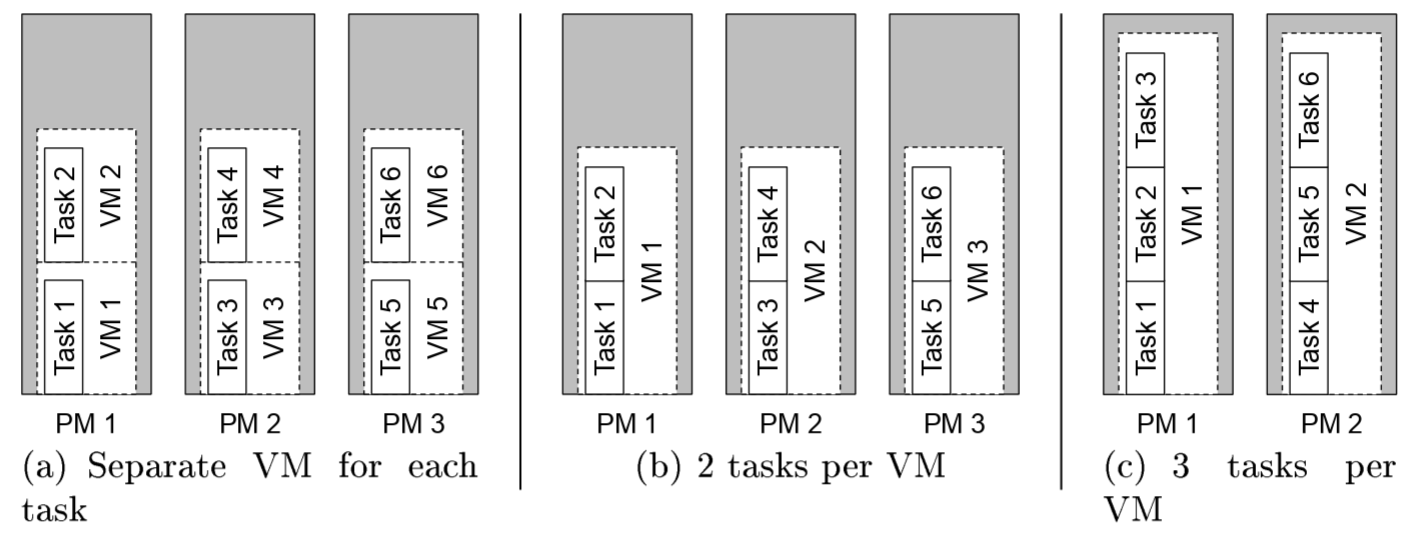
\includegraphics[width=0.8\textwidth]{example.png}
% 	\caption{An example shows VM multiplexing can reduce 33\% of energy consumption \cite{}}
% 	\label{fig:example}
% \end{figure}

% Another limitation of IaaS model is that it only provides limited types of VM with fixed amount resources (including CPU, memory, etc). When a customer chooses VM type, they are forced to
% choose a VM type with the enough resource of a critical resource (e.g. CPU), therefore, other resources are over-provisioned \cite{Gmach:2012uu}. In order to tackle the fixed size of resources,
% previous researchers employ an overbooking technique \cite{Tomas:2013us}, where extra
% VM can be placed in a PM dependent on the actual resource utilization in that PM instead of the VM sizes.

% As shown above, service allocation has strong influence on VM placement.
% Therefore, instead of considering of complicated algorithms to achieve server consolidation.
% We can think from system design point of view to build a cross-layer (SaaS and IaaS) 
% collaborative technique which leads to high utilization as well as energy saving. 

% Another benefit brought from this technique is that, it will further releases the burden from 
% server providers of estimating the resource requirement and resource selection. 
% The price model will follow the pay-as-you-go policy so that service providers do not need to 
% rent a certain amount of reserved resources to cover the minimum requirement.


% % \subsubsection*{Affinity aware VM Placement}
% \subsubsection*{VM Multiplexing}

% Another direction that could potentially improve the utilization of resource is VM multiplexing.
% VM multiplexing is a technique that several services are deployed into a same VM so that 
% it improve the utilization of saving a little amount of resource from running a separated VM.

% VM multiplexing is a technique that usually be conducted by a private cloud owner, because 
% private cloud owner has complete control of cloud resources and tasks, multiple tasks 
% can be consolidated in one VM. Previously, VM multiplexing is not suitable for a public cloud
% environment because the operating system cannot offer a performance isolation among the 
% applications running internally.

% With the prevalence of container technology (e.g Docker \cite{}), public cloud providers can
% offer isolated virtual environments with shared operating system 
% which is in essence VM multiplexing. 
% Containers can increase the efficiency of cloud resource 
% utilization because it is much light weighted than a VM which means it requires 
% much less resource to than a VM manager.  Additionally, containers share a single operating system,
% which offers much fast inter-container communication via system standard calls than inter-VM
% communication techniques.

% Current research mostly concentrate on VM consolidation problem. However, when the 



% % \subsubsection*{EC-based Dynamic VM Placement}
% % \subsubsection*{Large Scale of Server Consolidation Problem with Container}

% \section*{Research Goal}
% The overall goal of this thesis is to propose a server consolidation approach that
% considers the challenges from all six points mentioned 
% above when generating solutions.
% Specifically, this approach combines element of AI planning to ensure the correctness
% and constraint, and of Evolutionary Computation, 
% to evolve a population of near-optimal solution. 
% The research aims to determine a flexible way in which planning and EC can be combined to allow the creation of solution to solve consolidation problems.
% The research goal described above can be achieved by completing the following set of 
% objectives, which are intended to be used as research guides throughout this project.

% \begin{enumerate}
% 	\item First, develop an Evolutionary computation approach that to solve the 
% 	combination of service allocation and VM placement problem. 
% 	This objective has three sub-objectives:
% 	\begin{enumerate}
% 		\item \textit{Develop a formulation to capture the relationship between service allocation and VM placement.}
% 		\item \textit{Propose a representation which address this problem} 
% 		\item \itextit{Develop a multi-objective EC-based algorithm to resolve this problem.}
% 	\end{enumerate}

% 	\item Second, we would consider the multi-objective container-based consolidation problem with predefine VM types.
% 	\begin{enumerate}
% 		\item bla
% 		\item bla bla 
% 	\end{enumerate}

% 	\item Third, we would develop an EC based approach that considers the container-based consolidation problem
% 		with customized the VM types.
% 	\begin{enumerate}
% 		\item bla
% 		\item bla
% 	\end{enumerate}

% 	\item Fourth, we would develop an approach for the joint allocation container and VM. 
% 	\begin{enumerate}
% 		\item bla
% 		\item bla
% 	\end{enumerate}

% 	\item Fifth, we would consider the affinity-aware constraint in the consolidation
% 	problem.
% 	\begin{enumerate}
% 		\item bla
% 		\item bla
% 	\end{enumerate}

% 	\item Sixth, we would consider the co-location problem with aware the applications resource usage. 
% 	\begin{enumerate}
% 		\item bla
% 		\item bla
% 	\end{enumerate}

% 	\item Seventh, we would consider the large scale consolidation problem with
% 	centralized approach with a dimensionality reduction method.
% 	\begin{enumerate}
% 		\item bla
% 		\item bla
% 	\end{enumerate}

% \end{enumerate}

% \section*{Organization of Proposal}
% The remainder of the proposal is organized as follows: Chapter 2 provides a fundamental definition of the Server Consolidation problem and performs a literature review covering a range of works in this field; Chapter 3 discusses the preliminary work carried out to explore using  EC-based techniques for the integration of service allocation and VM placement problem, one of the objectives proposed in this project; Chapter 4 presents a plan detailing this project’s intended contributions, a project timeline, and a thesis outline.

% \emph{The third aspect} The dynamic 
% \textcolor{Maroon}{Brief Literature Review}

% In the previous decade, 
% Cloud providers who were focusing on ensuring quality of service, 
% has quickly expanded their infrastructures into a large scale.
% As a result, the average utilization of servers is as low as 20\%, 
% according to \cite{energy_2007}'s observation of google's datacenter, hence, the energy was largely wasted. 

% Despite the energy consumption by none information and communication technologies (ICT) equipments
% such as cooling and airing systems, 
% the energy can be derived from two aspects, first, the hardwares of servers contribute a static consumption. 
% Second, the usage of computing, storage and network resources cause a dynamic consumption. 
% Therefore, improving the efficiency of resources are also two folds, minimizing the static part and 
% delievering more performance proportional to the dynamic workload.

% These are the inituition behind server consolidation. Server consolidation improves the utilization of resources by 
% concentrates workloads in a few servers so that others can be turned off or put into sleep to save energy. 
% Therefore, it achieves reduction of static energy consumption as well as improving the utilization of resources. 
% The consolidation can be done with the help of virtual machine (VM), 
% which can be easily transport from one physical machine (PM) to another. 
% However, as the scale of reallocation of VMs become large and various quality of services (QoS) requirements have to
% be considered, an efficient automatic approach is an urgent and necessary need.